% !TEX root = ../main.tex
\chapter{Model creation} \label{ch:model}
% TITOLO DA VALUTARE

This chapter will outline the approach suggested by IBM Reserch for tackling some of the challanges introduced in \nameref{ch:introduction} regarding fault detection and diagnosis (FDD) and for overcoming the limitations of the state of the art approaches. A step-by-step example illustrating the approach is provided at the end of the chapter.

\section{State of the art}
Nowadays, as extensively analyzed by \textcite{methods_for_diagnostic}, FDD approaches fall in either one of the following three categories: physycal model based approaches, data driven approaches and rule-based approaches. Still, each of these approaches shares common limitations that can be summarized as:
\begin{itemize}
  \item they can only be applied to a single, specific building
  \item they require large manual effort and expertise
  \item their deployment can take several weeks
  \item they neglect strong interactions between systems.
\end{itemize}

\paragraph{Physycal model approach} \label{subsec:phy_models}
This approach requires a physycal model (e.g ordinary differential equations) of the building and its components. They are highly precise in diagnosing faults given a correct model. However, deriving the models is no trivial task and requires times and expertise. On top of this, derived models are building, system and location specific and they are difficult to adapt to other buildings than the one they are thought for, even if they share similar structure and similar components, thus limiting the scalability of this approach.

\paragraph{Data driven approach} \label{subsec:data_models}
Data driven approaches completely rely on building's sensor data. They assume that access to a large dataset of hystorical data is granted. There is little to no need for any a priori knowledge of the processes involved. Black-box data driven approaches derive the model in the form of an input-output relationship whose parameters are not correlated with the actual physical parameter (e.g artificial neural networks, regression) while grey-box data driven approaches take advantage of simplified physical relationships between measured quantities (e.g principal component analysys) and rely on statistical methods for estimating their parameters. Even though these methods do not suffer from scalability issues, they are limited to fault detection and lack in diagnosis capabilities.

\paragraph{Rule-based approach} \label{subsec:rule_models}
The rule-based approach is the most common in traditional FDD applications. It uses domain knowledge and expertise in order to derive a series of simple \textit{if-then-else} rules or some kind of decision trees along with a series of thresholds and confidence intervals; during system operations data are evaluated against this rules and countermeasures are eventually taken. Even though this is the most common approach, it still needs a lot of manual effort and requires access to domain knowledge so these requirements still limit portability and scalability of applications based on this technique.

\section{IBM Research approach}
The approach developed by IBM Research is based on a combination of the three aformentioned concepts to overcome their disadvantages. It models high level physical processes in the systems to derive diagnosis rules, it parametrizes the rules using data analytics techniques and applies them during system's operations. The strength of the semantic approach lies in its capability to automatically infer knowledge given a building, its sensors and their data. This leads to a semi-automated process that limits the manual effort needed, as shown in \autoref{fig:approach_overview}.
\begin{figure}
  \centering
  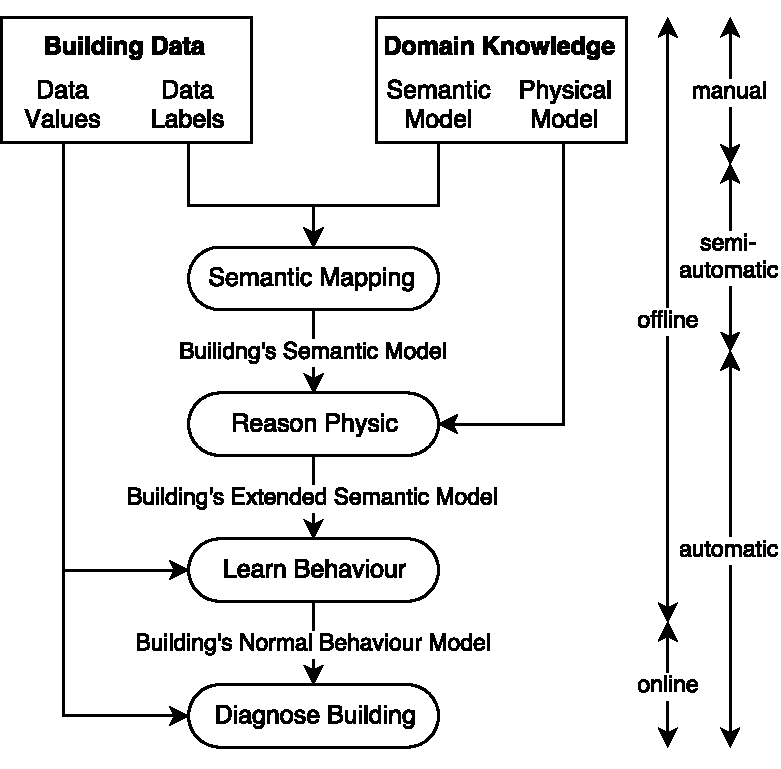
\includegraphics[width=0.7\textwidth]{approach_overview.pdf}
  \caption{IBM Reserch approach, overview}
  \label{fig:approach_overview}
\end{figure}

The proposed approach needs three inputs to produce the diagnosis of a given anomaly:
\begin{itemize}
  \item building data: assumed available in the building's Building Management System (BMS)
  \item semantic model: specified through the use of concepts from domain ontologies Brick (\autoref{subsec:brick}) and SSNO (\autoref{subsec:ssn})
  \item physycal model: the model of the physical dependencies between subsystems of the building. The physical processes are modelled through concepts presented in the extended SSNO. (\autoref{subsec:ssn}).
\end{itemize}
These inputs are processed through the various stages to produce the complete model of the building and its internal processes. Details about the different phases are given in the following pages.

\subsection{Semantic Mapping} \label{subsec:semantic_mapping}
Building a semantic model for a specific building needs knowledge on the type of sensors, meters and various equipment available in said building, their location and their semantic meaning in the chosen ontologies. These informations are usually stored in BMS through labels that, despite some kind of standardization efforts, are usually vendor specific; in some cases even the same vendor ends up changing its labelling schemes throughout the years. Even though there is no common ground to evaluate these labels, usually they are comprised of a series of abbreviations and acronyms, eventually separated by some special character (e.g ``\textunderscore'') that gives informations about the device's ID, function and location (or the equipment it is part of). An air temperature sensor in a room on ground floor can be labeled AIR\textunderscore TEMP\textunderscore R3GF while another air temperature sensor in a room on the first floor may ends up being labeled as RATSF1R9; both the sensors represent a common semantic resource in an ontology and need to be mapped to that concept. This process is called semantic mapping. Existing approaches are differentiated in three types\cite{semantic_mapping}:
\begin{itemize}
  \item semi-automatic: they offer a tool assisting the user in labelling the point to corresponding semantic types and are based on advanced text mining techniques (e.g regular expressions, classifiers)
  \item data driven: these approaches try to recover the meta-data given the timeseries. They are based on the concept that different data-points exhibiting similar timeseries behaviour should be similar themselves
  \item active feedback: in these kind of approaches a series of known events are injected into the system and datapoints semantic model is derived observing the effect of the event injection.
\end{itemize}

\subsubsection{Building Energy Asset Discovery tool}
the Building Energy Asset Discovery (BEAD) tool\cite{bead} is the tool developed by IBM Research for assisting user in the process of discovery and tagging of sensors. The tool is based on dictionaries of the type $\mathcal{D}:\mathcal{A}\rightarrow \mathcal{MS}$ where $\mathcal{A}$ is the set of all relevant acronyms and $\mathcal{MS}$ is the set of markerset; each markerset is a set of markers or keywords. These concepts are closely related to those of tagset and tag found in the Brick ontology and this duality allows the association of the sensor with the correct semantic type as described by Brick (see \autoref{subsec:brick}). The dictionary contains the most common acronyms found in BMS and it is further extended by the markers (tags) from the Brick ontology, such that a tag maps to itself, e.g Temperature$\rightarrow$\{Temperature\}. The tool takes a label from the BMS, computes a similarity score against the dictionary entries and guides the user in the labelling process. For example, given the following dictionary
\begin{description}[noitemsep]
  \item \textbf{d1}: RAT$\rightarrow$\{Return, Air, Temperature\}
  \item \textbf{d2}: RAT$\rightarrow$\{Room, Air, Temperature\}
  \item \textbf{d3}: SAT$\rightarrow$\{Supply, Air, Temperature\}
  \item \textbf{d4}: OAT$\rightarrow$\{Outdoor, Air, Temperature\}
  \item \textbf{d5}: Temp$\rightarrow$\{Temperature\}
  \item \textbf{d6}: Temperature$\rightarrow$\{Temperature\}
\end{description}
the label RATSF1R9 (Room Air Temperature Sensor, Floor 1, Room 9) has a high similarity with both RAT$\rightarrow$\{Return, Air, Temperature\} and RAT$\rightarrow$\{Room, Air, Temperature\}, so it is up to the user to understand the meaning and choose the right markerset. In a similar fashion, it is possible to extract information on the location of a sensor or the asset it is related to, as shown in \autoref{tab:bead_dictionary}.
\begin{table}
  \centering
  \caption{Dictionary extended with assets' informations}
  \label{tab:bead_dictionary}
  \begin{tabular}{lll}
    \hline
    \textbf{Label} & \textbf{Asset} & \textbf{Marketset}                       \\\cline{1-3}
    U6\textunderscore RAT        & AHU6  & \{Return, Air, Temperature\}    \\
    U6\textunderscore DAT        & AHU6  & \{Discharge, Air, Temperature\} \\
    AHU7\textunderscore RAT      & AHU7  & \{Return, Air, Temperature\}    \\
    AHU7\textunderscore SAT      & AHU7  & \{Supply, Air, Temperature\}    \\
    AU9\textunderscore RET\textunderscore TEMP & AHU9  & \{Return, Air, Temperature\}    \\
    AU9\textunderscore SUP\textunderscore TEMP & AHU9  & \{Supply, Air, Temperature\}
  \end{tabular}
\end{table}
This process clearly requires human supervision, hence the definition of semi-automatic, but through this approach the operator has to manually inspect a smaller subset of all the possible marketsets, thus taking minutes instead of several weeks to complete the semantic mapping. Practical experiments demonstrated that through this approach the decrease in number of labels to analyze is the 7.5\% of the total number of BMS labels \cite{semantic_mapping}.
The output of this process is the semantic model of the specific building according to the chosen ontology. A flowchart illustrating this process is shown in \autoref{fig:semantic_mapping}.

\begin{figure}
  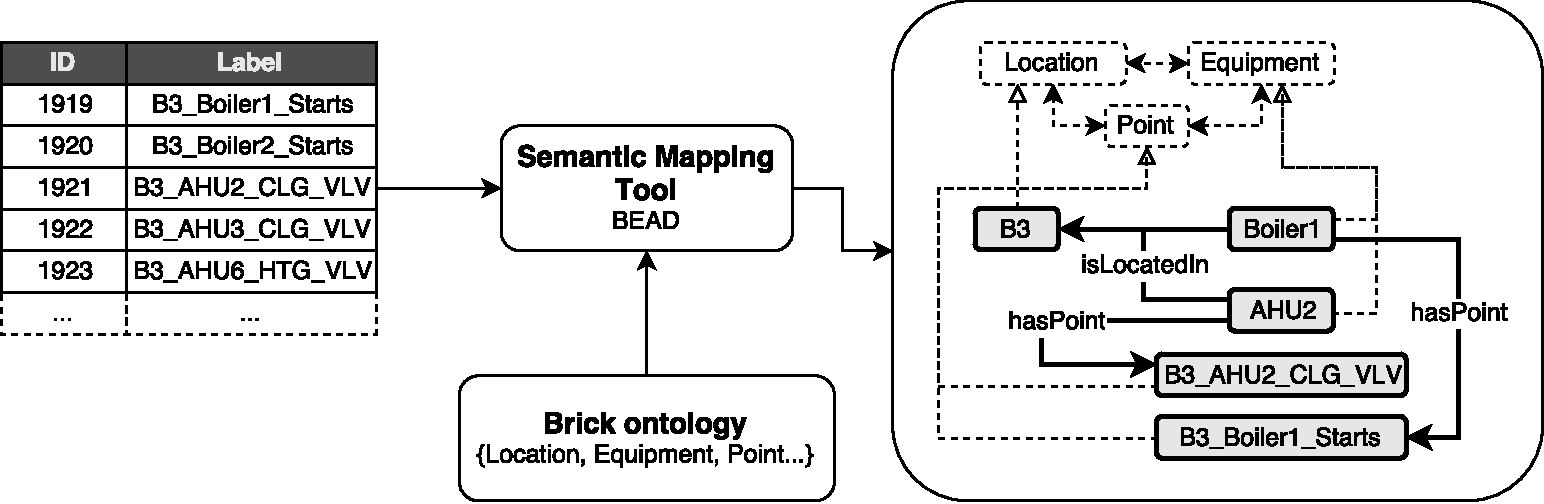
\includegraphics[width=1\textwidth]{semantic_mapping.pdf}
  \caption{Semantic mapping process}
  \label{fig:semantic_mapping}
\end{figure}

\subsection{Physic model inference}
The semantic model obtained from the semantic mapping phase is a model of the building architecture, assets, sensors and their loaction across the building. The model still lacks information about the physic processes taking place in the building and how the actual physic model is monitored and influenced by the points (sensors, setpoints etc.) in the building. Manually building the physical model of a building is unpractical and costly, thus the developed framework approaches this challange through the use of semantic inference techniques. This phase requires as inputs the semantic model of the building and an appropriate ontology that models the physics variables. Given those inputs, through the reasoning process is possible to automatically add the correct dependencies and physical processes to the model. This process is separated in two phases:
\begin{itemize}
  \item physical properties inference: it recreates the physical variables that are involved in physical processes. The properties are either mandatory or optional
  \item physical processes inference: once the physical properties are set in place, it is possible to link them together according to the domain knowledge specified in the upper ontology.
\end{itemize}
Further informations about the concept of reasoning and reasoner and further details about implementation choices for this approach are given in \autoref{ch:framework}.

\paragraph{Physical properties inference}
Properties represent physical quantities in the real world and can be mandatory or optional. Mandatory properties are characteristic of a ssn:FeatureOfInterest and need to be created for each instance of that feature. This behaviour is specified in the ontology of the physic through the use of the phy:requiresProperty relationship, so that during the reasoning mandatory properties can be automatically created. For example, in \autoref{fig:properties} it is shown that the concept of :Room phy:requiresProperty :Temperature, that means that every instance of a :Room needs to be associated with a property that is an instance of :Temperature, or in plain English that every room has a temperature.
\begin{figure}
  \centering
  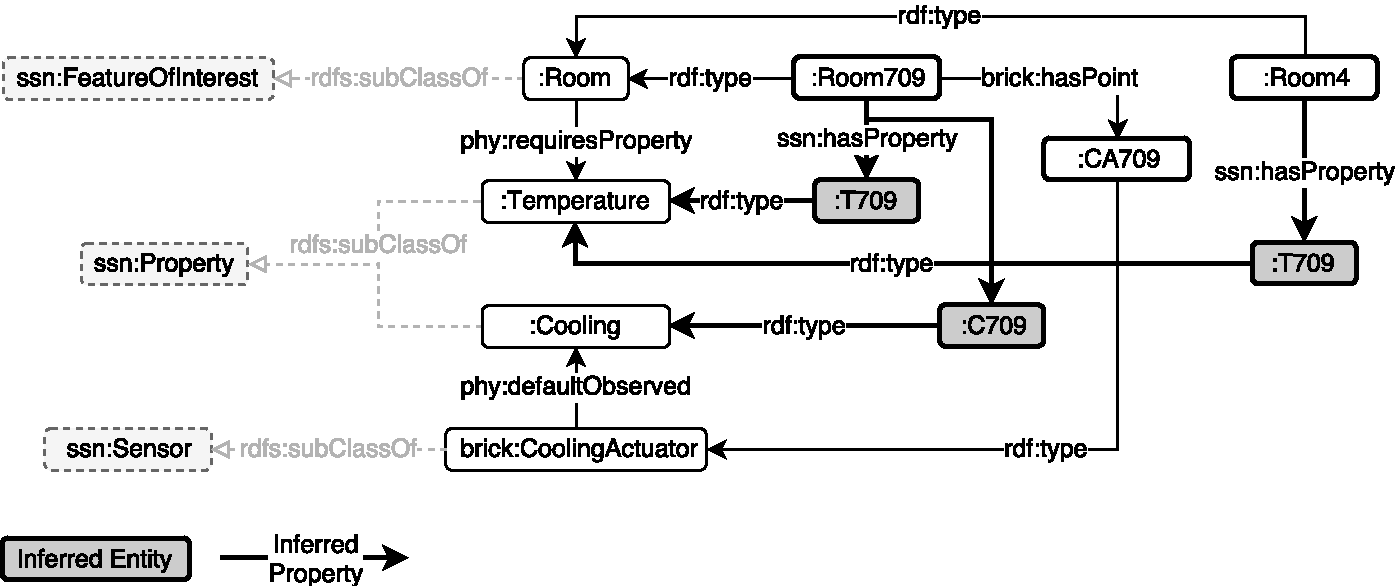
\includegraphics[width=1\textwidth]{properties.pdf}
  \caption{Process of inference of mandatory and optional properties}
  \label{fig:properties}
\end{figure}
Optional properties, on the other hand, need to be created only if some requirements are met, for example a :Room have a :Cooling property only if a :CoolingActuator is present in said room, and it is modelled in the ontology as :CoolingActuator phy:defaultObserved :Cooling. In \autoref{fig:properties} it can be seen that only :Room709 has a :Cooling property since it is the only room that has a :CoolingActuator.
The :requiresProperty and :defaultObserved properties\footnote{Intended as the semantic concept of relationship between entities, not to be confused with domain knwoledge properties like :Temperature.} are concept level references and model general knowledge. General knowledge describes the domain without bothering about the ground truth. This means, for example, that the concept of :Room requires the existance of the concept of :Energy even if there are no rooms instances in the building's model. The existence of said properties is the key for the automatic reasoning process.

\paragraph{Physical processes inference}
Once all the actual properties have been infered for a specific configuration, it is time to append to the model informations about the physical processes involving such properties. As already stated in \autoref{subsec:ssn}, physical processes are modelled as Linear Time Invariant (LTI) systems based on the fact that Multiple Input Multiple Output (MIMO) processes can be decomposed into multiple Multiple Input Single Output (MISO) processes
  \begin{gather*}
        \dot{x}=A\cdot x+B\cdot u \\
        y=C\cdot x+D\cdot u
  \end{gather*}
that splitted on the output rows and in case of indipendent inputs becomes
\begin{equation}
  y_i=\sum_{j \in J}\Bigg[\sum_{l\in L_j}c_{i,l}\cdot x_l+\sum_{k\in K_j}d_{i,k}\cdot u_k\Bigg]=\sum_{j \in J}f_{i,j}(u_j)
\end{equation}
A MISO process can be further subclassed as a Single Input Single Output process.
Each process follows the rules
\begin{description}[noitemsep]
  \item\textbf{Rule 1} a process has at least one input and exactly one output
  \item\textbf{Rule 2} when a process has multiple inputs, they superpose additively.
\end{description}
Given these rules, it is possible to define a class hierarchy of LTI processes that are used to model a physical system. A subset of said taxonomy is available at \autoref{tab:lti_taxonomy}.
\begin{table}
  \centering
  \caption{Taxonomy of the semantic representation of LTI processes}
  \label{tab:lti_taxonomy}
  \begin{tabular}{lll}\hline
    \textbf{Semantic concept} & \textbf{Parent} & \textbf{Formal definition} \\\hline
    MISO & Process & $y_i(t)=\bm{c_i}\cdot \bm{x_i}+\bm{d_i}\cdot \bm{u_i}(t)=f(\bm{u}(t))$ \\\hline
    SISO & MISO & $y_i(t)=\bm{c_i}\cdot \bm{x_i}+d_i\cdot u_i(t)=f(u(t))$ \\\hline
    Positive Correlted (PC) & SISO & $y(t)\propto u(t)$ \\
    Negative Correlated (NC) & SISO & $y(t)\propto -u(t)$ \\
    Proportional (P) & SISO & $y(t)=k_p\cdot u(t)$ \\
    Positive Proportional (PP) & PC, P & $y(t)=k_p\cdot u(t), k_p\geq 0$\\
    Negative Proportional (NP) & NC, P & $y(t)=k_p\cdot u(t), k_p<0$\\
    Negation (N) & NP & $y(t)=k_p\cdot u(t), k_p=-1$\\
    Integral (I) & P & $y(t)=k_I\int u(t)dt$\\
    Derivative (D) & P & $y(t)=k_D\cdot\dot u(t)$\\
    Lag (PTn) & P & $\sum_{i=0}^{n}C_i\cdot T^i \cdot y^{(i)}(t)=k_{PT}\cdot u(t) $\\
    1\textsuperscript{st} order lag (PT1) & PTn & $T\cdot\dot y(t)+y(t)=k_{PT}\cdot u(t)$\\
    Delay ($\tau$) & SISO & $y(t)=u(t-\tau), \tau>0$\\
    Multiplicative (M) & MISO & $y(t)=u_1(t)\cdot u_2(t)$
  \end{tabular}
\end{table}

\subsection{Learning the normal behaviour}\label{subsec:learn_behaviour}
This phase is not strictly related to the ones detailed in the previous sections in this chapter, yet it is of utmost importance for the diagnosis process. This phase allows for the definition of general rules that represent a confidence interval of the normal behaviour of the sensors. These rules are derived from different statistical and machine learning methods. \textcite{inproceedings_cognitive_buildings} suggest the use of Artificial Neural Networks (ANN) for modelling the temperature comfort in a room. Generalized Addictive Models (GAM) can be used for modelling energy processes so that a subsequent Autoregressive Moving Avarage (ARMA) model can characterize the normal behaviour\cite{e2d}. The approach determines a series of upper and lower bounds that characterize the normality interval for a given sensor. Behaviours outside these ranges are classified as anomaly and they trigger the diagnosis phase. Studying this methods is outside the scope of the thesis and so these confidence intervals are assumed to be known without bothering about how they were derived.

\section{Example of the whole approach}\label{sec:full_example}
In order to better explain the concepts presented in the previous sections, it is provided an example of the full process applied to a room, facing the outside environment, with a cooling Air Handling Unit (AHU). At the end of the section it is shown that a full model of the room and its internal and external processes are derived. This model will then be used during the explanation of the diagnosis process. Looking back at \autoref{fig:approach_overview}, we start by defining the inputs needed for the process (sharp top boxes).
\paragraph{Building data and semantic model}
It is assumed that some kind of BMS is available in the building so that through the BMS is it possible to retrieve both labels (for semantic mapping) and data of various sensors.
The room analyzed in the example will be named ROOM1. In ROOM1 an air temperature sensor and an occupancy sensor are available. Room1 is also equipped with an AHU, named AHU709, whose internal components are observed by a fan mode sensor, a supply air flow sensor a coil water temperature sensor and a coil water flow sensor. This AHU709 is fed by a chiller named C1 equipped with a power sensor. Let the BMS contain the data as in \autoref{tab:bms_example} and lets use Brick (\ref{subsec:brick}) as a domain ontology.
\begin{table}
  \centering
  \caption{Example of BMS content}
  \label{tab:bms_example}
  \begin{tabular}{l|l}
    \hline
    \textbf{ID} & \textbf{Label} \\\hline\hline
    1234 & CCPC1B3 \\\hline
    1235 & CWFU709 \\\hline
    1236 & CWTU709 \\\hline
    1237 & SAFAHU709C1 \\\hline
    1238 & FMAHU709 \\\hline
    1239 & OCCR1 \\\hline
    1240 & ATSROOM1 \\\hline
    1241 & ATS\textunderscore Outside \\\hline
  \end{tabular}
\end{table}
Through the semantic mapping tool (\autoref{subsec:semantic_mapping}) it is possible to map the labels in the BMS to the Semantic type in the Brick ontology. The user can also give the system additional informations about the architecture of the building and the location of equipments and sensors. It is then possible to map :B3 as a brick:Location, :ROOM1 still as brick:Location and then link one to the other as :ROOM1 brick:isPartOf :B3 and so on. The tool will also discover the semantic type of the sensor and will be able to create the correct instances. For example it will add to the model an air temperature sensor named :ATSROOM1 and will link it as a point to :ROOM1. The output semantic graph can be seen in \autoref{fig:semantic_mapping_example} where the instances created from the BMS and their mutual relationships are bold, while the Brick ontology concepts and relationships are light grey. This is the building semantic model, that will be used together with the physic model described in the next paragraph to infer knowledge about the physics properties and relationships in the building.
\begin{figure}
  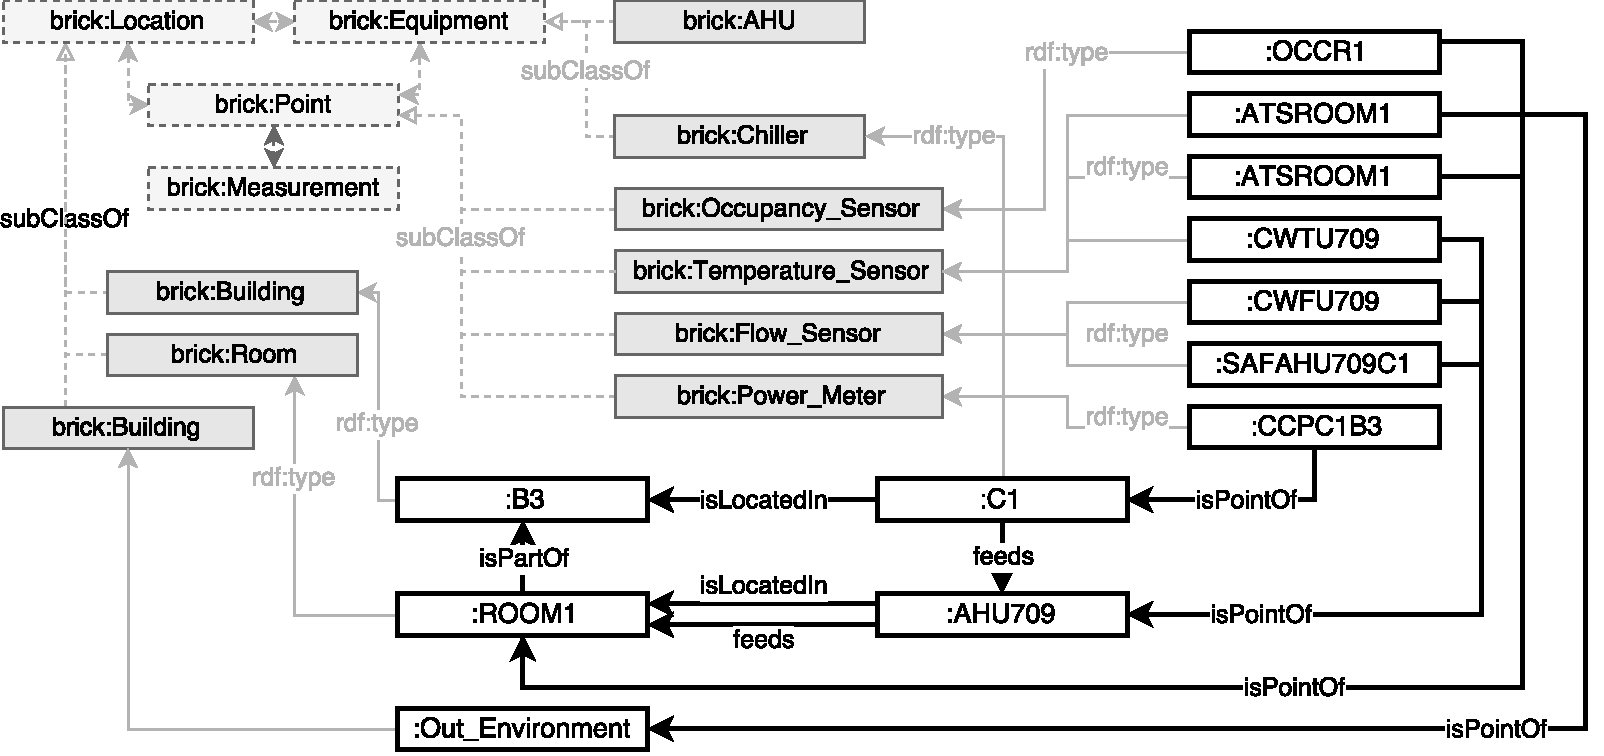
\includegraphics[width=1\textwidth]{semantic_mapping_example.pdf}
  \caption{Complete semantic model of a room in a building equipped with an AHU according to Brick ontology}
  \label{fig:semantic_mapping_example}
\end{figure}

\paragraph{Physic model}
The physic model is a model of the physic phenomena occuring in an enviroment. It defines physical variables and processes and their interaction in the context of a specific domain. Creating a model of physic's laws is a time consuming task that involves expertise from different fields, from engineering to physics, that are very domain specific. The good side of the semantic approach is that, once the model is derived from a general point of view, it is automatically extended for every instance of a building, indipendently from its architecture. It is to note that the domain model for the physic does not necessarily model exact physical relationships but just the principal ones, since those are the most relevant to the approach. However this choice is purely practical rather then a limitation of the approach itself, and given sufficient time and knowledge, it is possible to enrich the model in order to close the gap with the reality. Here will be presented a model for the physic of a room, equipped with a AHU fed by a chiller. The model is based on a simplification that makes the assumption of fully mixed air, that allows for the modelling of a whole space as a single node with uniform temperature. \textcite{building_room_physics} provides an insight of the physics involved in the example. It starts describing a heat balance equation of a room as
\begin{gather}
  m_rc_p\dot{\vartheta_{r}}=Q_{Energy}\label{eq:room_variables}\\
  Q_{Energy}=Q_{Occ}+Q_{Cool}+\sum{A_ih_i(\vartheta_{i}-\vartheta_{r})}\label{eq:energy_composition}\\
\end{gather}
and from \autoref{eq:room_variables} and \autoref{eq:energy_composition} it derives
\begin{equation}
  m_rc_p\dot{\vartheta_{r}}+\sum{A_ih_i\vartheta_{r}}=Q_{Occ}+Q_{Cool}+\sum{A_ih_i\vartheta_{i}} \label{eq:room_lag}
\end{equation}
that says that the temperature of a room $\vartheta_r$ is a first order derivative of the room's inner energy $Q_{Energy}$ that is the combination of the heat gain of occupants $Q_{Occ}$, the heat removed by the cooling system $Q_{Cool}$ and the heat transfer between adjacent environments. Given these equations, semantic informations can be extracted.
From \autoref{eq:room_variables} it can be seen that
\begin{enumerate}[noitemsep]
  \item rooms have an internal energy [Property, mandatory]
  \item rooms have a temperature [Property, mandatory]
\end{enumerate}
while from \autoref{eq:energy_composition} it follows that
\begin{enumerate}[noitemsep, resume]
  \item a room's temperature is influenced by the energy in a first order lag process [Process, PT1]
  \item rooms can be cooled, if they have a cooling actuator [Property, optional]
  \item cooling is negative proportional (NP) with the room's energy
  \item room energy depends from the adjacents enviroment's temperature proportional to the shared surface $A_i$ and the heat transfer coefficient $h_i$, hence the dependency is a positive proportional process [Process, PP].
\end{enumerate}
Further analyzing the physics involved bring to the conclusion that
\begin{equation}
  Q_{Occ}=q_{lat}n_{occ} \label{eq:occupancy_heat}
\end{equation}
where $q_{lat}$ is the latent heat gain and $n_{occ}$ the number of occupants in the room. From  \autoref{eq:energy_composition} and \autoref{eq:occupancy_heat} it follows that
\begin{enumerate}[noitemsep, resume]
  \item rooms have a number of occupants [Property, Mandatory]
  \item a room's internal energy is positively correlated with the number of occupants [Process, PP].
\end{enumerate}
Additional knowledge can be added if the physics of the system in known; for example, it is possible to further enrich the model by specifying the internal processes that regulate a AHU. \textcite{building_ahu_physics} provide a simplified model for modelling the cooling load of an AHU through \autoref{eq:cooling_load}
\begin{equation}
  Q_{Cool}=\frac{c_a\dot{m_{a}^{e}}c_c\dot{m_{c}^{e}}}{c_{a}\dot{m_{a}^{e}}+c_c\dot{m_{c}^{e}}}(\vartheta_{a}-\vartheta_{c}) \label{eq:cooling_load}
\end{equation}
This, given that $\vartheta_a$ is the mixed air temperature, $\dot{m_a}$ the air flow rate, $\vartheta_c$ the chilled water temperature and $\dot{m_c}$ the chilled water flow rate, leads to the following conclusions
\begin{enumerate}[noitemsep, resume]
  \item cooling is a complex function of the air temperature, the chilled water temperature, the supply air flow and the water flow in the coil [Process, MISO].
\end{enumerate}
Finally, \textcite{building_chiller_physics} provide a simple model of a chiller's physics, whose equation can be expressed as
\begin{equation}
  \dot{m_c}c_w(\vartheta_{cret}-\vartheta_c)=\eta_{COP}W
\end{equation}
from which it can be derived that
\begin{enumerate}
  \item the chilled water tempearture decreases with the increase of the power consumption [Process, NP]
  \item the water flow rate increases as the power consumption of the pump increases [Process, PP].
\end{enumerate}
\begin{figure}
  \begin{subfigure}[b]{.6\textwidth}
    \centering
      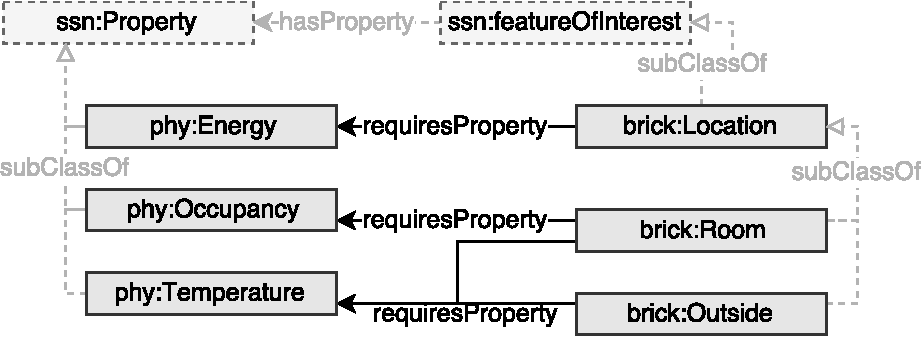
\includegraphics[width=1\linewidth]{mandatory_properties.pdf}
      \caption{Mandatory properties}
      \label{fig:mandatory_properties}
  \end{subfigure}
  \begin{subfigure}[b]{.4\textwidth}
    \centering
      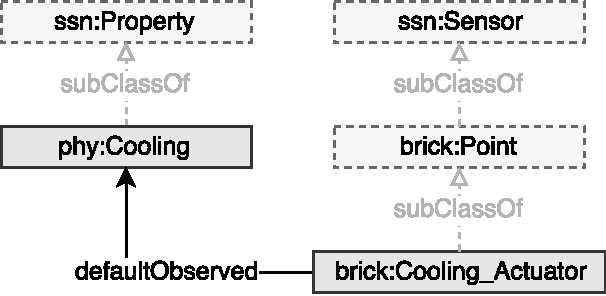
\includegraphics[width=1\linewidth]{optional_properties.pdf}
      \caption{Optional properties}
      \label{fig:optional_properties}
  \end{subfigure}
  ~
  \centering
  \begin{subfigure}[b]{.5\textwidth}
    \centering
      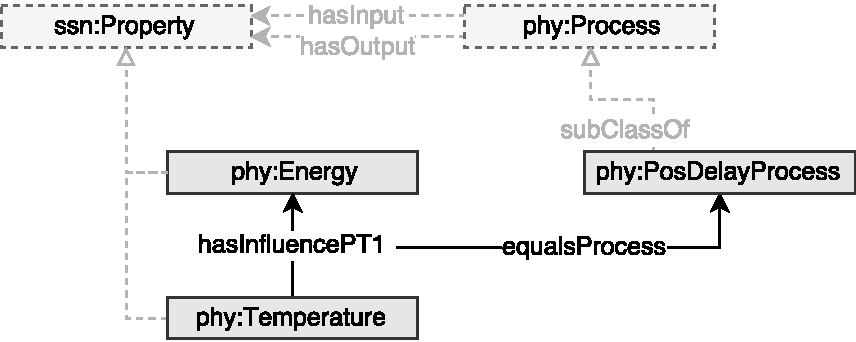
\includegraphics[width=1\linewidth]{processes_definition.pdf}
      \caption{Process}
      \label{fig:processes_definition}
  \end{subfigure}
  \caption{Patterns for definition of a model for a system's physics}
  \label{fig:physic_model}
\end{figure}
This dependencies can be semantically mapped to a domain ontology that still use concept from Brick, SSN and its extended version and \autoref{fig:physic_model} shows how the discovered domain knowledge can be represented using those ontologies.
It is clear that this part is the most costly of the whole process, especially timewise, since it requires very specific expertise. In the example, for instance, it is not captured that a room's internal energy is influenced by the radiant heat of the sun but it would have been possible to do so. The good side of this approach is that the modelling efforts need to be done just once per domain as the ontology is reusable and will adjust itself to the bulding instance trough the automatic reasoning process.

\paragraph{Reasoning process}
The reasoning process is divided in two main phases: the discovery of the physical properties and the creation of the physical processes involving those properties. This requires access to the building semantic model created during the semantic mapping phase and the physic model derived by expert for the particular domain (e.g physic model of HVAC system). Both the phases work on the ontology (metadata) to draw conclusions about the instances. The first phase has to be the properties discovery one, since those properties are inputs and outputs for the processes. Based on the ontology derived in the previous paragraph and the semantic model of the building (\autoref{fig:semantic_mapping_example}), through the application of simple reasoning rules, it is possible to derive the whole semantic graph of both the building and its actual physic beahviour, as seen in \autoref{fig:ex_building_full}, in a simplified form\footnote{Since even the degree of complexity of the semantic graph of small example is too high, the fidelity to the real graph is dropped for clairty's sake.}.
The rules to be applied are:
\begin{itemize}
  \item if there is a room, it has an internal energy, $Room(r)\Rightarrow Energy(e)\land hasProperty(r,e)$
  \item if there is a room, it has a temperature, $Room(r)\Rightarrow Temperature(t)\land hasProperty(r,t)$
  \item if there is a temperature sensor in a room, the room has a temperature and the temperature is observed by the sensor, $Room(r)\land Temperature\_Sensor(ts)\land hasPoint(r,ts)\Rightarrow Temperature(t)\land hasProperty(r,t)\land observes(s,t)$
  \item energy influences the temperature through a PT1 process, $Room(r)\land Energy(e)\land hasProperty(r,e)\land Temperature(t)\land hasProperty(r,t)\Rightarrow PT1(p)\land hasInput(p,e)\land hasOutput(p,t)$
  \item energy of a room depends on the outside temperature if they are adjacent, $Room(r)\land Outside(o)\land isNextTo(r,o)\land Temperature(t)\land hasProperty(o,t)\land Energy(e)\land hasProperty(r,e)\Rightarrow PP(p)\land hasInput(p,t)\land hasOutput(p,e)$
  \item if a AHU has a coil water flow sensor then it has a coil water flow property, $AHU(a)\land CoilWaterFlowSensor(s)\land hasPoint(a,s)\Rightarrow CoilWaterFlow(f)\land hasProperty(a,f)\land observes(s,f)$.
\end{itemize}
\begin{figure}
  \centering
  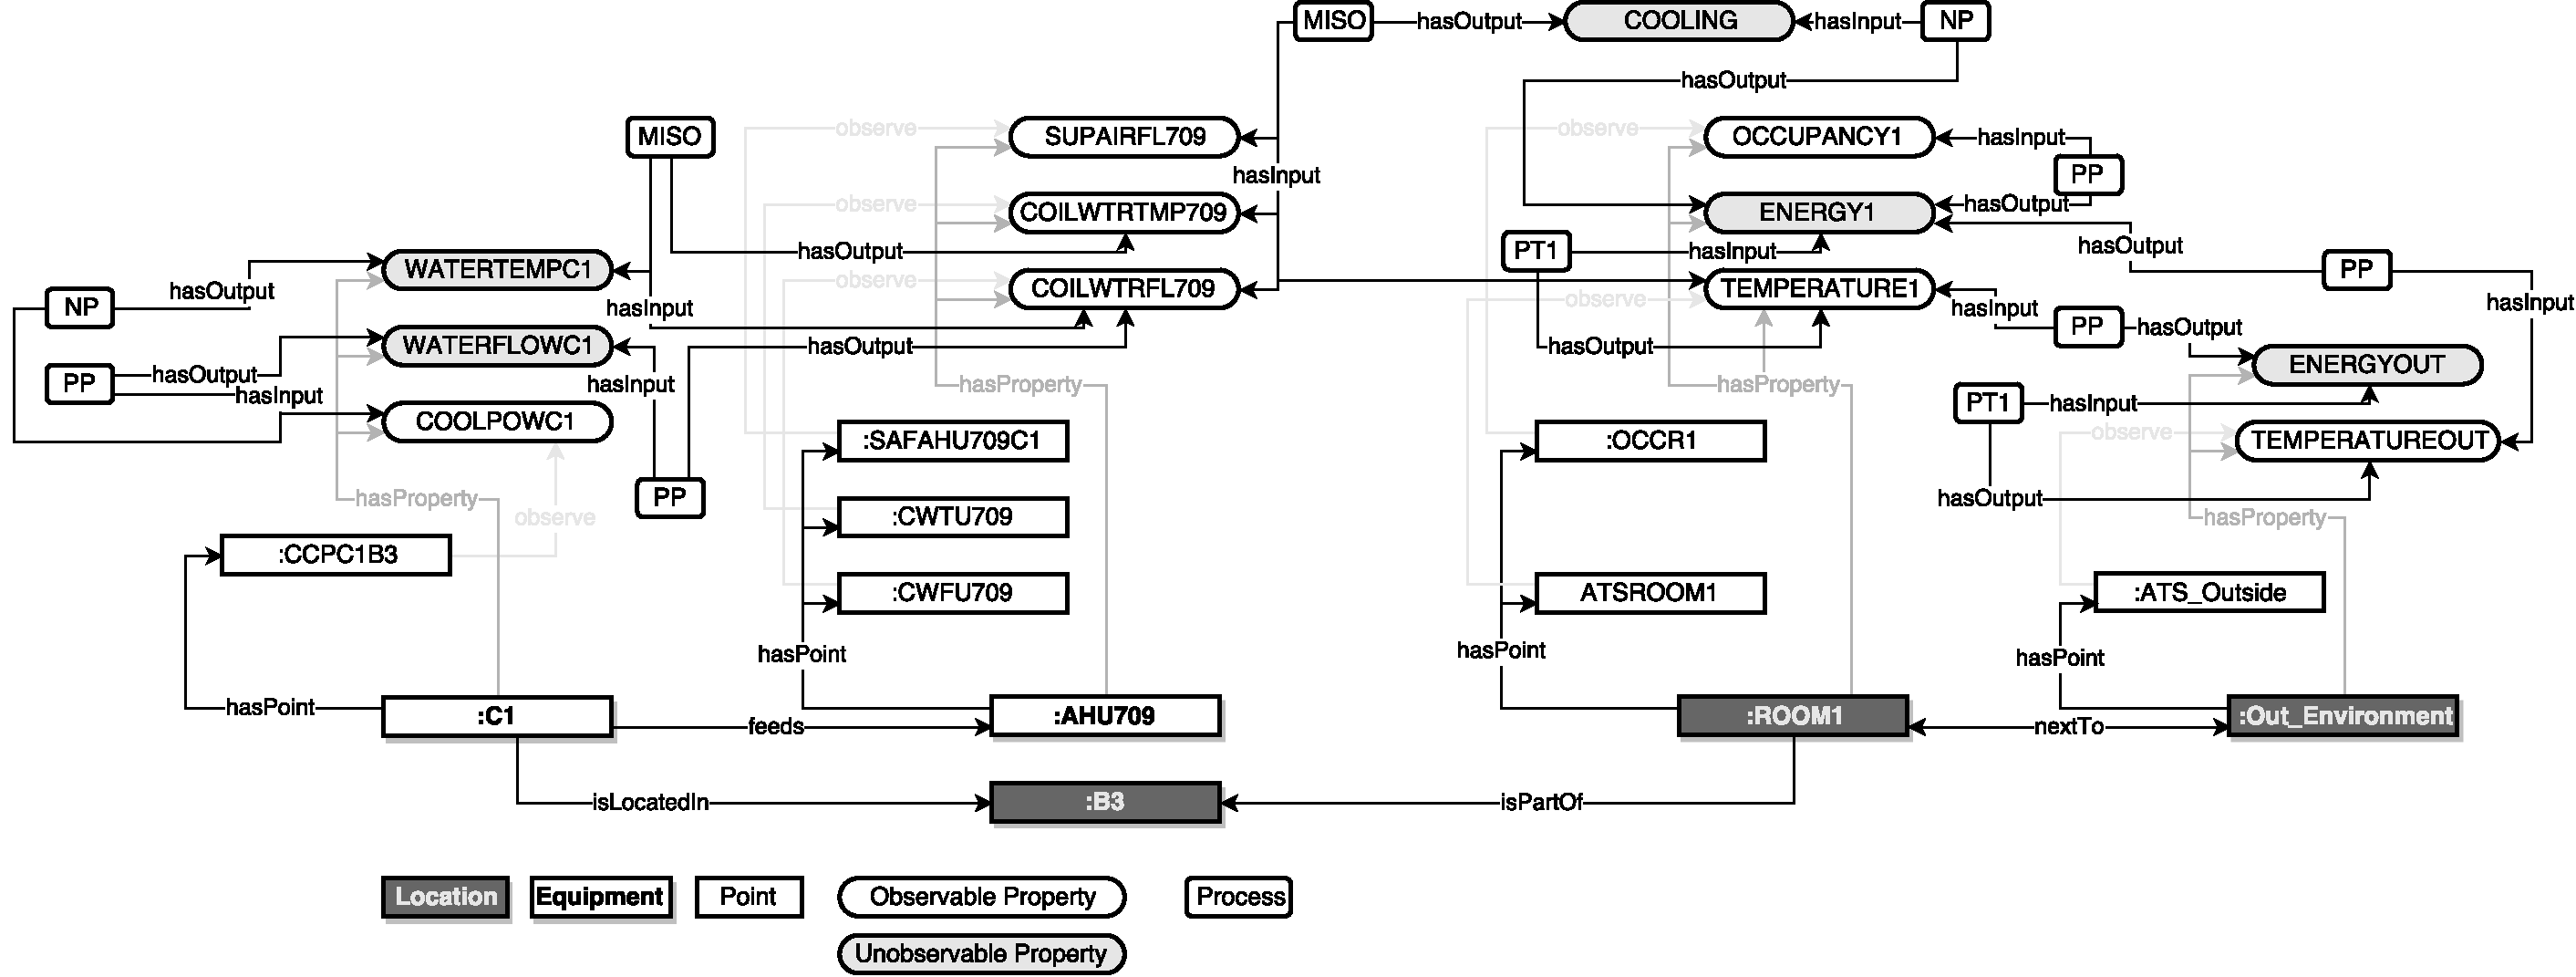
\includegraphics[width=.95\textheight, angle=90, keepaspectratio]{example_full.pdf}
  \caption{Semantic model of the building and its physics}
  \label{fig:ex_building_full}
\end{figure}
The reasoning rules can be completed for the remaining AHU's components reusing similar patterns as those shown in the list above.
These inference rules are explicitly written as implications among instances (no ontological reasoning is involved) because it is easier to convey the concept this way and, since this example is really small, it was easy and fast enough to be done by hand. Even a slightly more complex example would have required a more refined reasoning scheme involving the concepts, the instances and their mutual relationships. However it is already possible to get a grasp of the portability of this approach just noticing that, just with these simple rules, it does not matter how many instances of rooms, AHUs or chillers there can be. The reasoner would still enforce the correct properties in an automatic fashion.
Looking back at the examples in this chapter, it can be noticed that, even in a small example, there are many informations encoded in the graph that starts to grow in size and complexity. Therefore it starts to surface one of the challanges of this approach, addressed in \autoref{ch:framework}, that is the scalability issue for big commercial buildings.
